\documentclass{article}
\usepackage[margin=1in]{geometry}
\usepackage{../common}
\usepackage{../pagesetup}

\begin{document}
%\lecture{**LECTURE-NUMBER**}{**DATE**}{**LECTURER**}{**SCRIBE**}
\lecture{2}{September 6}{Sasha Rush}{Anna Sophie Hilgard, Diondra Peck}{Discrete Models}

\begin{itemize}
\item Discrete models take values from a countable set, e.g. \{0,1\}, \{cold, flu, asthma\} and are simpler than continuous models.
\item We will use simple discrete models to develop our tactics such as marginalization and conditioning. 
\item Today, we will focus coins as a real-world example.
\end{itemize}

\subsection{Bernoulli model}
The likelihood is of the form $p(\text{heads}) = \theta$.

\subsubsection*{Easy Prior}
Assume we know the coin came from one of 3 unknown manufacturers (later, we'll have mixture model estimation, but for now assume these probabilities come from an oracle).
\begin{enumerate}
\item $\theta = 0.4$ with probability .1
\item $\theta = 0.5$ with probability .8
\item $\theta = 0.6$ with probability .1
\end{enumerate}

$$p(\theta) = 0.1 \cdot \delta(\theta = 0.4)  + 0.8 \cdot \delta(\theta = 0.5) + 0.1 \cdot \delta(\theta = 0.6)$$

\subsubsection*{Likelihood}
Likelihood = $p(\text{data}|\text{parameters})$. For the coin example, 
$$p(\text{coin flips}|\theta) = \textrm{Bin}(N_1 | N, \theta) = {\binom{N}{N_1}} \theta^{N_1} (1-\theta)^{N-N_1} \quad \text{where $N = N_0 + N_1 =$ number of flips}$$

\noindent Note that the last two terms, the "score", is our focus since they are the only terms that depend on $\theta$. The first term normalizes the distribution.

\subsection{Inference}
Inference 1: $p(\theta|x)$ ($x \in N_0, N_1$). How can we estimate $\theta$?

\subsubsection*{Maximum Likelihood Estimation (MLE)}
\begin{align*}
\theta_{MLE} &= \textrm{argmax}_{\theta} \; p(N_0,N_1 | \theta) = \textrm{argmax}_{\theta}  \;\textrm{log}\left[p(N_0,N_1 | \theta)\right] \\
\theta_{MLE} &= \textrm{argmax}_{\theta} \;\textrm{log}{\binom{N}{N_1}} + N_1 \textrm{log} \theta + N_0  \textrm{log} (1-\theta)\quad \text{Because the first term is not a function of $\theta$, we can ignore it.} \\
\frac{d}{d\theta} &= \frac{N_1}{\theta} + \frac{N_0}{1-\theta} \cdot ( -1)  \rightarrow \theta_{MLE} = \frac{N_1}{N_0 + N_1} \\
\end{align*}

\noindent Note that Inference $\neq$ Decision Making. If we asked you to make a bet on the coin, based on this you could either
\begin{enumerate}
\item Always take heads if $\theta > .5$. In this case, $p(\text{win}) = \theta$
\item Take heads with probability = $\theta$. In this case, $p(\text{win}) = \theta^2 + (1-\theta)^2$ [p(\text{is heads}) * p(\text{choose heads}) + ...]
\end{enumerate}
If $\theta$ = 0.6, for option 1, p(\text{win}) = $\theta$ = 0.6. For option 2, p(\text{win}) = $\theta^2 + (1 - \theta)$ = 0.52. In this case, the additional information used in the calculation of option 2 does not result in a better decision.


\subsubsection*{Maximizing the Posterior (MAP)}
Bayes Rule : $p(\theta|\text{data}) \propto p(\text{data}|\theta) p(\theta)$
\begin{itemize}
\item Posterior: $p(\theta | \text{x})$
\item Likelihood: $p(\text{x} | \theta)$
\item Prior: $p(\theta)$
\end{itemize}
$$\theta_{MAP} = \textrm{argmax}_{\theta} \; p(\theta | \text{x}) = \textrm{argmax}_{\theta}  \;\textrm{log}\left[p(\text{x} | \theta) p(\theta)\right] \quad \text{from Bayes' Rule:  $p(\theta | \text{x}) \propto p(\text{x} | \theta) p(\theta)$}$$

\smallskip

\noindent Consider an example:
\begin{align*}
p(\theta=0.4|N_0,N_1) &\propto {\binom{N}{N_1}} (.4)^{N_1}(1-.4)^{N_0} (0.1) \\
p(\theta=0.45|N_0,N_1) &= 0 \quad \text{Due to the sparsity of the prior - similar result for $\theta$ = 0.5 and 0.6}
\end{align*}
\noindent $\theta_{MAP} = \theta_{MLE}$ when we have a uniform prior since the MLE calculation does not explicitly factor a prior into its calculation.

\subsubsection*{Full Posterior}
Partition or Marginal Likelihood: $p(N_0,N_1) = \int_\theta p(N_0,N_1,\theta)$. 
\begin{align*}
p(\theta|N_0,N_1) &= \frac{p(x|\theta) p(\theta)}{p(N_0,N_1)} && \text{Note that $p(N_0,N_1)$ is a very difficult term to compute.}
\end{align*}

\subsubsection*{Beta Prior}
\begin{align*}
p(\theta|\alpha_0,\alpha_1) = \frac{\Gamma(\alpha_0 + \alpha_1)}{\Gamma(\alpha_0)\Gamma(\alpha_1)} \theta^{\alpha_1-1} (1-\theta)^{\alpha_0-1}  && \text{support $\in [0,1]$}
\end{align*}

\noindent From the image of the beta function for different parameters, we can see that it can ether be balanced, skewed to one side, or tend toward infinity on one side.
\begin{figure}
\centering
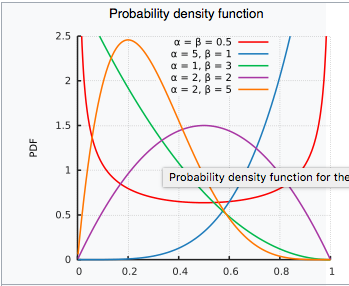
\includegraphics[width=0.5\textwidth]{./beta.png}
\caption{Beta Params}
\end{figure}

\smallskip

\noindent With a beta prior: 
\begin{align*}
p(\theta|N_0,N_1) &= \frac{\Gamma(\alpha_0 + \alpha_1)}{\Gamma(\alpha_0)\Gamma(\alpha_1)} \theta^{\alpha_1-1} (1-\theta)^{\alpha_0-1} \theta^{N_1}(1-\theta)^{N_0} \cdot \textrm{(constant normalization term w.r.t $\theta$)} 
\end{align*}

\noindent The key insight is that we get additive terms in the exponent and the resulting distribution looks like another beta. The prior "counts'' (pseudocounts) from the hyperparameters can be interpreted as counts we have beforehand. \\

\begin{align*}
p(\theta|N_0,N_1) = \frac{\Gamma(\alpha_0 + \alpha_1)}{\Gamma(\alpha_0)\Gamma(\alpha_1)} \theta^{N_1 + \alpha_1-1} (1-\theta)^{N_0 + \alpha_0-1} \cdot \textrm{(constant normalization term w.r.t $\theta$)}
\end{align*}

\noindent To make this distribution sum to 1, use the known beta normalizer
\begin{align*}
p(\theta|N_0,N_1) = \frac{\Gamma(\alpha_0 + \alpha_1 + N_0 + N_1)}{\Gamma(\alpha_0)\Gamma(\alpha_1)\Gamma(N_0)\Gamma(N_1)} \theta^{N_1 + \alpha_1-1} (1-\theta)^{N_0 + \alpha_0-1} \sim \textrm{Beta}(\theta | N_0 + \alpha_0, N_1 + \alpha_1) \quad \text{(posterior)}
\end{align*}
\noindent The mode of the Beta gives us back $\theta_{MAP}$, but with additional information about the shape of the distribution. What does the prior that tends to infinity at 1 imply? That in the absence of other information, the coin is definitely heads.

\subsubsection*{Predictive Distribution}
\begin{align*}
p(\hat{x}| N_0, N_1) &= \int_\theta p(x|\theta, N_0, N_1) p(\theta | N_0, N_1) d\theta \\
&= \int_\theta \theta p(\theta | N_0, N_1) d\theta \\
&= \E_{\theta \sim p(\theta|N_0, N_1)} \theta
\end{align*}
\noindent This is the expectation under the posterior of $\theta$ which is the  mean of the Beta distribution. Feel free to prove this as an exercise.

\subsubsection*{Marginal Likelihood}
\begin{align*}
p(N_0, N_1) &= \int_\theta p(x_1, \hdots x_n | \theta) p(\theta) d\theta \\
&= \int_\theta \frac{\Gamma( \alpha_1 +  \alpha_1)}{\Gamma(\alpha_0)\Gamma(\alpha_1)} \theta^{\alpha_1 + N_1 -1} (1-\theta)^{\alpha_0+N_0-1}
\end{align*}

\noindent The first term can be moved outside, as it does not depend on $\theta$. After introducing our normalization term and making the distribution insidesum to 1,

\begin{align*}
p(N_0, N_1) = \frac{\Gamma( \alpha_1 +  \alpha_1)}{\Gamma(\alpha_0)\Gamma(\alpha_1)} \frac{\Gamma(N_0 + \alpha_0)\Gamma(N_1 + \alpha_1)}{\Gamma(N_0 + N_1 + \alpha_0 + \alpha_1)}
\end{align*}

\subsection{Extensions on the Coin Flip Model: Super Coins}
\begin{itemize}
\item Many correlated coins: models of binary data, important for discrete graphical models
\item Many-sided coins aka dice: models of categorical data, generalization of Bernoulli
\end{itemize}

\subsection{Other Distributions}
\begin{align*}
\textrm{Bernoulli}(x|\theta) &= \theta^{x}(1-\theta)^x \\
\textrm{Categorical}(x|\theta) &= \prod_k\theta_k^{x_k} && \text{generalization of Bernoulli} \\
\textrm{Multinomial}(x|\theta) &= \frac{(\sum x_k) !}{\prod_k x_k!}\prod_k\theta_k^{x_k} && \text{generalization of Binomial} \\
\textrm{Dirichlet}(x|\alpha) &= \frac{\Gamma(\sum \alpha_k)}{\prod \Gamma(\alpha_k)}\prod_k\theta_k^{\alpha_k-1} && \text{generalization of Beta, often used as a prior}
\end{align*}

\noindent Note that the Dirichlet distribution is the conjugate prior of the Categorical and Multinomial distributions.

\subsection{Example notebook}
See \href{https://github.com/harvard-ml-courses/cs281-demos/blob/master/Beta.ipynb}{Beta.ipynb}
\end{document}